\documentclass{article}
\usepackage[spanish,es-tabla]{babel}
\usepackage{graphicx} % Required for inserting images
\usepackage[spanish]{babel}
\usepackage{float}
\usepackage{amsmath}
\usepackage{hyperref}
\usepackage{adjustbox}

\hypersetup{
	colorlinks=true,
	urlcolor=blue,
	linkcolor=black,
}

\begin{document}

\begin{titlepage}
	\centering
	{\LARGE Universidad de Santiago de Compostela}\\
	\vspace{1.5cm}
	{\Large Escuela Técnica Superior de Ingeniería}\\
	\vspace{3cm}
	{\Huge Práctica 3}\\
	\vspace{0.5cm}
	\bigskip
	{\large Fundamentos de sistemas paralelos\\ \today}\\
	\vspace{3cm}
	{\Large \textit{Pablo Liste Cancela - David Corral Pazos}}
	\vfill
\end{titlepage}

\section{Introducción}

	% TODO

\section{Entorno de ejecución}

	% TODO

\subsection{Consideraciones}

	% TODO
	% Por si acaso, que somos gallegos

\section{Ejercicio 1}

	\subsection{Introducción}

		En este apartado se analizan las características técnicas de diferentes unidades de procesamiento gráfico (GPUs) empleadas para computación de alto rendimiento, utilizando la biblioteca CUDA. El objetivo es extraer y comprender las propiedades específicas de las GPUs disponibles en el CESGA (Centro de Supercomputación de Galicia), así como de una GPU local para establecer comparaciones.

		Para ello usaremos el programa \textit{devquery.cu}, basado en funciones proporcionadas por CUDA, permite obtener detalles clave sobre las GPUs, como su capacidad de cómputo, configuraciones de hardware, recursos disponibles por multiprocesador y bloque, así como parámetros relacionados con el rendimiento de la memoria. Estos datos son fundamentales para optimizar aplicaciones que hacen uso intensivo de GPUs, como en inteligencia artificial, simulaciones físicas y análisis de datos.

		Además de las unidades instaladas en el supercomputador del CESGA, NVIDIA T4 y NVIDIA A100, también se ha probado a ejecutar el programa en las máquinas personales de los integrantes del equipo. Esto ha permitido obtener resultados adicionales para los modelos NVIDIA GTX 1070 y NVIDIA GTX 1050 TI. De esta manera, se puede comparar no solo las características de las GPUs diseñadas específicamente para computación de alto rendimiento (HPC), sino también las propiedades de GPUs de uso general, más enfocadas en aplicaciones de consumo como videojuegos o diseño gráfico. Este análisis resulta útil para entender las diferencias clave entre arquitecturas orientadas a diferentes segmentos del mercado y sus posibles aplicaciones así como para visualizar la evolución técnica a lo largo del tiempo.

	\subsection{Resultados obtenidos}

		Una vez completado el código fuente original, añadiendo la visualización de todos los elementos requeridos (como el número de SMs, hilos por bloque, entre otros), se procedió a ejecutar el programa para obtener los resultados. Los datos obtenidos fueron registrados en archivos de texto y posteriormente comparados con los valores técnicos oficiales proporcionados en la \href{https://cesga-docs.gitlab.io/ft3-user-guide/gpu_nodes.html}{documentación del CESGA}. Este proceso permitió validar la precisión de los resultados y garantizar la fiabilidad de las observaciones realizadas.

		\begin{table}[H]
			\centering
			\begin{tabular}{|l|l|}
				\hline
				\textbf{Propiedad} & \textbf{Valor} \\ \hline
				Device name & NVIDIA A100-PCIE-40GB \\ \hline
				Major revision number & 8 \\ \hline
				Minor revision number & 0 \\ \hline
				Multiprocessor count & 108 \\ \hline
				Max threads per SM & 2048 \\ \hline
				Max dimension size of a thread block (x, y, z) & (2147483647, 65535, 65535) \\ \hline
				Max threads per block & 1024 \\ \hline
				Max dimension size of a block (x, y, z) & (1024, 1024, 64) \\ \hline
					Registers per SM & 65536 \\ \hline
				Registers per block & 65536 \\ \hline
				Shared memory per multiprocessor (bytes) & 167936 \\ \hline
				Shared memory per block (bytes) & 49152 \\ \hline
				Total global memory (bytes) & 42298834944 \\ \hline
				Memory clock rate (Hz) & 1215000 \\ \hline
				Memory bus width (bits) & 5120 \\ \hline
				Peak memory bandwidth (GB/s) & 1555.20 \\ \hline
				Number of CUDA cores & 6912 \\ \hline
			\end{tabular}
			\caption{Propiedades de la GPU NVIDIA A100-PCIE-40GB}
		\end{table}

		\begin{table}[H]
			\begin{tabular}{|l|l|}
				\hline
				\textbf{Propiedad} & \textbf{Valor} \\ \hline
				Device name & Tesla T4 \\ \hline
				Major revision number & 7 \\ \hline
				Minor revision number & 5 \\ \hline
				Multiprocessor count & 40 \\ \hline
				Max threads per SM & 1024 \\ \hline
				Max dimension size of a thread block (x, y, z) & (2147483647, 65535, 65535) \\ \hline
				Max threads per block & 1024 \\ \hline
				Max dimension size of a block (x, y, z) & (1024, 1024, 64) \\ \hline
					Registers per SM & 65536 \\ \hline
				Registers per block & 65536 \\ \hline
				Shared memory per multiprocessor (bytes) & 65536 \\ \hline
				Shared memory per block (bytes) & 49152 \\ \hline
				Total global memory (bytes) & 15655829504 \\ \hline
				Memory clock rate (Hz) & 5001000 \\ \hline
				Memory bus width (bits) & 256 \\ \hline
				Peak memory bandwidth (GB/s) & 320.064 \\ \hline
				Number of CUDA cores & 2560 \\ \hline
			\end{tabular}
			\centering
			\caption{Propiedades de la GPU Tesla T4}
		\end{table}

		\begin{table}[H]
			\begin{adjustbox}{width=\textwidth, keepaspectratio}
				\begin{tabular}{|l|l|}
					\hline
					\textbf{Propiedad} & \textbf{Valor} \\ \hline
					Device name & NVIDIA GeForce GTX 1070 \\ \hline
					Major revision number & 6 \\ \hline
					Minor revision number & 1 \\ \hline
					Multiprocessor count & 15 \\ \hline
					Max threads per SM & 2048 \\ \hline
					Max dimension size of a thread block (x, y, z) & (2147483647, 65535, 65535) \\ \hline
					Max threads per block & 1024 \\ \hline
					Max dimension size of a block (x, y, z) & (1024, 1024, 64) \\ \hline
						Registers per SM & 65536 \\ \hline
					Registers per block & 65536 \\ \hline
					Shared memory per multiprocessor (bytes) & 98304 \\ \hline
					Shared memory per block (bytes) & 49152 \\ \hline
					Total global memory (bytes) & 8589672448 \\ \hline
					Memory clock rate (Hz) & 4004000 \\ \hline
					Memory bus width (bits) & 256 \\ \hline
					Peak memory bandwidth (GB/s) & 256.256 \\ \hline
					Number of CUDA cores & 1920 \\ \hline
				\end{tabular}
			\end{adjustbox}
			\centering
			\caption{Propiedades de la GPU NVIDIA GeForce GTX 1070}
		\end{table}

		\begin{table}[H]
			\begin{adjustbox}{width=\textwidth, keepaspectratio}
				\begin{tabular}{|l|l|l|l|}
					\hline
					\textbf{Propiedad} & \textbf{NVIDIA A100} & \textbf{Tesla T4} & \textbf{GTX 1070} \\ \hline
					Device name & NVIDIA A100-PCIE-40GB & Tesla T4 & NVIDIA GeForce GTX 1070 \\ \hline
					Major revision number & 8 & 7 & 6 \\ \hline
					Minor revision number & 0 & 5 & 1 \\ \hline
					Multiprocessor count & 108 & 40 & 15 \\ \hline
					Max threads per SM & 2048 & 1024 & 2048 \\ \hline
					Max dimension size of a thread block (x, y, z) & (2147483647, 65535, 65535) & (2147483647, 65535, 65535) & (2147483647, 65535, 65535) \\ \hline
					Max threads per block & 1024 & 1024 & 1024 \\ \hline
					Max dimension size of a block (x, y, z) & (1024, 1024, 64) & (1024, 1024, 64) & (1024, 1024, 64) \\ \hline
					Registers per SM & 65536 & 65536 & 65536 \\ \hline
					Registers per block & 65536 & 65536 & 65536 \\ \hline
					Shared memory per multiprocessor (bytes) & 167936 & 65536 & 98304 \\ \hline
					Shared memory per block (bytes) & 49152 & 49152 & 49152 \\ \hline
					Total global memory (bytes) & 42298834944 & 15655829504 & 8589672448 \\ \hline
					Memory clock rate (Hz) & 1215000 & 5001000 & 4004000 \\ \hline
					Memory bus width (bits) & 5120 & 256 & 256 \\ \hline
					Peak memory bandwidth (GB/s) & 1555.20 & 320.064 & 256.256 \\ \hline
					Number of CUDA cores & 6912 & 2560 & 1920 \\ \hline
				\end{tabular}
			\end{adjustbox}
			\centering
			\caption{Propiedades de las GPUs: NVIDIA A100, Tesla T4 y GTX 1070}
		\end{table}

	\subsection{Comparación de resultados}

		A continuación se presenta un análisis detallado de las principales propiedades de las tres GPUs evaluadas: NVIDIA A100, Tesla T4 y GTX 1070. La comparación incluye la justificación de las diferencias observadas en cada propiedad y su implicación en el rendimiento y la aplicación en diferentes tipos de tareas.

		\subsubsection{Capacidad de cómputo (\textit{Major/Minor Revision Number})}

			\begin{table}[H]
				\begin{adjustbox}{width=\textwidth, keepaspectratio}
					\begin{tabular}{|l|l|l|l|}
						\hline
						\textbf{Propiedad} & \textbf{NVIDIA A100} & \textbf{Tesla T4} & \textbf{GTX 1070} \\ \hline
						Major revision number & 8 & 7 & 6 \\ \hline
						Minor revision number & 0 & 5 & 1 \\ \hline
					\end{tabular}
				\end{adjustbox}
				\centering
				\caption{Compute capabilities de las GPUs: NVIDIA A100, Tesla T4 y GTX 1070}
			\end{table}

			Las capacidades de cómputo (\textit{compute capabilities}) son un factor crítico al evaluar GPUs para diferentes aplicaciones. Estas capacidades, definidas por NVIDIA, indican las funcionalidades de hardware soportadas por una GPU en la arquitectura CUDA, lo que afecta directamente su rendimiento y eficiencia en tareas específicas. A continuación, se presenta un análisis detallado basado en los datos de la tabla proporcionada, complementado con información técnica relevante sobre el hardware.

			Las capacidades de cómputo (\textit{compute capabilities}) de una GPU, expresadas a través de los valores de \textit{Major revision number} y \textit{Minor revision number}, son determinantes para identificar las características arquitectónicas que soportan. Estas versiones marcan la compatibilidad con funciones específicas de CUDA y la eficiencia en su ejecución. A continuación, se analiza cómo estas capacidades posicionan a la NVIDIA A100, Tesla T4 y GTX 1070 en términos de su evolución tecnológica.

			La NVIDIA A100, con un \textit{Major revision number} de 8 y un \textit{Minor revision number} de 0, pertenece a la arquitectura \textbf{Ampere}. Esta versión representa un salto significativo respecto a generaciones anteriores, incluyendo soporte para funciones avanzadas en CUDA 11, como la aceleración mejorada para operaciones de precisión mixta y optimizaciones específicas para modelos de aprendizaje profundo. El número de revisión menor, siendo 0, indica que es una implementación inicial dentro de su generación.

			La Tesla T4, con un \textit{Major revision number} de 7 y un \textit{Minor revision number} de 5, forma parte de la arquitectura \textbf{Turing}. Este número mayor refleja la generación inmediatamente anterior a \textbf{Ampere}, con soporte para CUDA 10 y características específicas como la integración de Tensor Cores. El número de revisión menor, relativamente alto, indica mejoras iterativas en esta generación, optimizando su desempeño en tareas específicas como la inferencia en inteligencia artificial.

			Por su parte, la GTX 1070, con un \textit{Major revision number} de 6 y un \textit{Minor revision number} de 1, se basa en la arquitectura Pascal. Este nivel de revisión evidencia una tecnología más madura en comparación con generaciones previas, pero limitada respecto a arquitecturas más recientes. Su compatibilidad se restringe a CUDA 9 y carece de funciones avanzadas disponibles en \textbf{Turing} y \textbf{Ampere}, como los Tensor Cores y soporte para operaciones de precisión mixta.

			En resumen, los números de revisión reflejan claramente la evolución de las capacidades de cómputo en estas GPUs. La NVIDIA A100 lidera con un diseño orientado a maximizar el rendimiento en aplicaciones modernas, la Tesla T4 equilibra eficiencia y funcionalidad en tareas especializadas, mientras que la GTX 1070, aunque adecuada para escenarios generales, es tecnológicamente más limitada. Estos valores proporcionan una base para entender las capacidades arquitectónicas antes de considerar otros aspectos como memoria o rendimiento específico.

		\subsubsection{Número de multiprocesadores (SMs)}

			\begin{table}[H]
				\begin{adjustbox}{width=\textwidth, keepaspectratio}
					\begin{tabular}{|l|l|l|l|}
						\hline
						\textbf{Propiedad} & \textbf{NVIDIA A100} & \textbf{Tesla T4} & \textbf{GTX 1070} \\ \hline
						Multiprocessor count & 108 & 40 & 15 \\ \hline
					\end{tabular}
				\end{adjustbox}
				\centering
				\caption{SMs de las GPUs: NVIDIA A100, Tesla T4 y GTX 1070}
			\end{table}

			El número de multiprocesadores (SM, \textit{Streaming Multiprocessors}) en una GPU es un indicador clave de su capacidad para procesar tareas en paralelo. Cada SM contiene núcleos CUDA, unidades de memoria compartida y otros recursos que permiten manejar miles de hilos simultáneamente. A continuación, se analiza cómo el recuento de SMs diferencia a las NVIDIA A100, Tesla T4 y GTX 1070 en términos de su arquitectura y rendimiento potencial.

			La NVIDIA A100, con 108 SMs, lidera en este aspecto, representando una GPU diseñada para maximizar el paralelismo. Este número significativamente alto permite a la A100 procesar una gran cantidad de operaciones concurrentes, ideal para tareas de cómputo masivamente paralelo como el entrenamiento de modelos de aprendizaje profundo, simulaciones científicas y aplicaciones en inteligencia artificial. Su elevado conteo de SMs, combinado con las optimizaciones arquitectónicas de Ampere, proporciona una capacidad sin precedentes para manejar cargas de trabajo complejas y escalables.

			La Tesla T4, con 40 SMs, tiene un diseño más equilibrado, orientado a aplicaciones específicas como la inferencia en aprendizaje profundo y el procesamiento de datos. Aunque posee menos SMs que la A100, su arquitectura \textbf{Turing} optimiza la eficiencia en tareas paralelas, combinando el rendimiento de los SMs con el soporte para Tensor Cores. Este número de multiprocesadores es adecuado para tareas intensivas pero menos exigentes en términos de paralelismo extremo, como la virtualización de escritorios o el análisis de video en tiempo real.

			Por su parte, la GTX 1070, con 15 SMs, refleja una arquitectura diseñada principalmente para aplicaciones generales y de consumo, como juegos y tareas gráficas. Este número limitado de SMs, característico de la arquitectura Pascal, permite un paralelismo suficiente para estas aplicaciones, pero resulta menos eficiente en escenarios que requieren una gran cantidad de hilos concurrentes, como el cómputo científico o la inteligencia artificial. A pesar de ello, la GTX 1070 sigue siendo una opción funcional para usuarios que no necesitan capacidades avanzadas de cómputo paralelo.

		\subsubsection{Hilos por multiprocesador (\textit{Max threads per SM})}

			\begin{table}[H]
				\begin{adjustbox}{width=\textwidth, keepaspectratio}
					\begin{tabular}{|l|l|l|l|}
						\hline
						\textbf{Propiedad} & \textbf{NVIDIA A100} & \textbf{Tesla T4} & \textbf{GTX 1070} \\ \hline
						Max threads per SM & 2048 & 1024 & 2048 \\ \hline
					\end{tabular}
				\end{adjustbox}
				\centering
				\caption{Hilos por SM de las GPUs: NVIDIA A100, Tesla T4 y GTX 1070}
			\end{table}

			La cantidad máxima de hilos por multiprocesador (\textit{Max threads per SM}) es un parámetro fundamental para evaluar la capacidad de una GPU en el manejo simultáneo de tareas en paralelo dentro de un único SM. Este valor determina cuántos hilos puede ejecutar un SM de forma concurrente, lo que afecta directamente el nivel de paralelismo y el rendimiento en aplicaciones CUDA. A continuación, se analiza este aspecto en las GPUs NVIDIA A100, Tesla T4 y GTX 1070.

			La NVIDIA A100 y la GTX 1070 comparten una capacidad máxima de 2048 hilos por SM. Este límite alto refleja un diseño orientado a maximizar el paralelismo dentro de cada multiprocesador, permitiendo manejar múltiples tareas simultáneamente con una alta eficiencia. En el caso de la A100, este valor se complementa con la gran cantidad de SMs disponibles, lo que amplifica aún más su capacidad para gestionar cargas de trabajo masivas. Por otro lado, en la GTX 1070, aunque la cantidad de hilos por SM es equivalente, el menor número de SMs reduce el número total de hilos que la GPU puede manejar en conjunto, limitando su rendimiento en comparación con arquitecturas más modernas.

			En contraste, la Tesla T4 soporta un máximo de 1024 hilos por SM, un valor que es la mitad del de las otras dos GPUs. Este límite más bajo está alineado con el diseño de la arquitectura \textbf{Turing}, que prioriza la eficiencia energética y el rendimiento en tareas específicas, como la inferencia en inteligencia artificial y el procesamiento multimedia. Aunque el número de hilos por SM es menor, la Tesla T4 optimiza su rendimiento mediante características avanzadas como Tensor Cores y un manejo eficiente de recursos para aplicaciones intensivas, pero de menor escala en términos de paralelismo.

			En resumen, la NVIDIA A100 y la GTX 1070 sobresalen en cuanto a la capacidad de paralelismo máximo por SM, lo que las hace adecuadas para aplicaciones que dependen de un número elevado de hilos concurrentes. Sin embargo, mientras que la A100 aprovecha al máximo esta capacidad con su elevado número de SMs, la GTX 1070 está más limitada por su diseño general. Por otro lado, la Tesla T4, aunque con un menor número de hilos por SM, optimiza el uso de recursos para aplicaciones específicas, sacrificando el paralelismo extremo en favor de la eficiencia y el rendimiento en tareas más delimitadas.

		\subsubsection{Dimensiones del bloque de hilos (\textit{Thread Block})}

			\begin{table}[H]
				\begin{adjustbox}{width=\textwidth, keepaspectratio}
					\begin{tabular}{|l|l|l|l|}
						\hline
						\textbf{Propiedad} & \textbf{NVIDIA A100} & \textbf{Tesla T4} & \textbf{GTX 1070} \\ \hline
						Max dimension size of a thread block (x, y, z) & (2147483647, 65535, 65535) & (2147483647, 65535, 65535) & (2147483647, 65535, 65535) \\ \hline
						Max dimension size of a block (x, y, z) & (1024, 1024, 64) & (1024, 1024, 64) & (1024, 1024, 64) \\ \hline
					\end{tabular}
				\end{adjustbox}
				\centering
				\caption{Dimensiones de los bloques de hilos de las GPUs: NVIDIA A100, Tesla T4 y GTX 1070}
			\end{table}

			Las dimensiones máximas de los bloques de hilos en CUDA definen los límites estructurales del paralelismo que una GPU puede soportar. Estas propiedades, compartidas entre la NVIDIA A100, Tesla T4 y GTX 1070, reflejan la capacidad del hardware para organizar los hilos en estructuras tridimensionales, optimizando así la ejecución de tareas paralelas. A continuación, se analizan estas características en detalle.

			El tamaño máximo de las dimensiones de un \textit{grid} está dado por ($X$, $Y$, $Z$), siendo (2147483647, 65535, 65535) para las tres GPUs. Este límite extremadamente alto para la dimensión $X$, combinado con valores significativos para $Y$ y $Z$, permite definir grillas con millones de bloques de hilos. Este diseño es uniforme en las arquitecturas \textbf{Ampere}, \textbf{Turing} y \textbf{Pascal}, asegurando compatibilidad para tareas masivas distribuidas en grillas extensas. Sin embargo, en aplicaciones reales, el número de bloques suele limitarse por otros factores como la memoria o los recursos físicos disponibles en la GPU.

			El tamaño máximo de un bloque de hilos es de (1024, 1024, 64) para las tres GPUs. Esto significa que un bloque puede contener hasta
			$1024  1024  64$ hilos, aunque en la práctica, el límite total es de 1024 hilos debido a restricciones de hardware. Estas dimensiones permiten una organización flexible de los hilos en aplicaciones tridimensionales, como simulaciones físicas o procesamiento de imágenes. Este límite uniforme refleja una estandarización en las arquitecturas CUDA, lo que facilita la portabilidad de los códigos entre diferentes generaciones de GPUs.

			Aunque las tres GPUs comparten estos límites, su capacidad para utilizarlos de manera eficiente varía dependiendo de otros factores, como el número de multiprocesadores y la cantidad máxima de hilos por SM. Por ejemplo, la NVIDIA A100, con su mayor número de SMs e hilos por multiprocesador, puede manejar de manera más efectiva aplicaciones que exploten estas dimensiones máximas. En contraste, la GTX 1070, con menos SMs y recursos limitados, puede alcanzar estos límites en casos más restringidos. La Tesla T4, aunque eficiente para tareas específicas, también está limitada por su menor cantidad de hilos por SM.

			Las dimensiones máximas de bloques y grillas son uniformes en las GPUs NVIDIA A100, Tesla T4 y GTX 1070, lo que garantiza una compatibilidad general en aplicaciones CUDA. Sin embargo, la capacidad práctica para aprovechar estos límites depende del hardware subyacente, como el número de SMs y la cantidad de hilos por SM. La A100, con sus especificaciones superiores, se posiciona como la más apta para manejar configuraciones extremas, mientras que la GTX 1070 y la Tesla T4 son más adecuadas para aplicaciones de menor escala o con requerimientos específicos.

		\subsubsection{Hilos por bloque (\textit{Max threads per block})}

			\begin{table}[H]
				\begin{adjustbox}{width=\textwidth, keepaspectratio}
					\begin{tabular}{|l|l|l|l|}
						\hline
						\textbf{Propiedad} & \textbf{NVIDIA A100} & \textbf{Tesla T4} & \textbf{GTX 1070} \\ \hline
						Max threads per block & 1024 & 1024 & 1024 \\ \hline
					\end{tabular}
				\end{adjustbox}
				\centering
				\caption{Hilos por bloque de las GPUs: NVIDIA A100, Tesla T4 y GTX 1070}
			\end{table}

			La cantidad máxima de hilos por bloque es un parámetro que define el límite superior de hilos que pueden organizarse dentro de un único bloque en una GPU. Este valor es crítico para estructurar el paralelismo en aplicaciones CUDA, ya que afecta directamente la capacidad de organizar las tareas en bloques para optimizar el rendimiento. En el caso de las GPUs NVIDIA A100, Tesla T4 y GTX 1070, este límite es idéntico, siendo 1024 hilos por bloque.

			El valor de 1024 hilos por bloque es un estándar en arquitecturas CUDA, desde Pascal hasta Ampere. Esto facilita la portabilidad del código CUDA entre distintas generaciones de GPUs, ya que los desarrolladores no necesitan ajustar este parámetro dependiendo del hardware. Este límite también es consistente con el diseño de los multiprocesadores (SMs), que están optimizados para manejar este número máximo de hilos de manera eficiente.

			Aunque el límite de 1024 hilos por bloque es el mismo para las tres GPUs, la capacidad práctica para utilizarlos varía según las características del hardware. La NVIDIA A100, con 108 SMs y un mayor número de hilos por multiprocesador (2048), tiene una ventaja en el manejo de múltiples bloques que utilicen este límite máximo, permitiendo una mayor eficiencia en aplicaciones que demandan un alto paralelismo.

			La Tesla T4, aunque eficiente en aplicaciones específicas como inferencia de aprendizaje profundo, está restringida a 1024 hilos por multiprocesador, lo que limita su capacidad para manejar múltiples bloques configurados al máximo simultáneamente. Por su parte, la GTX 1070, con menos SMs y recursos generales más modestos, puede encontrar cuellos de botella en aplicaciones que requieren una alta densidad de bloques con el límite máximo de hilos.

			La uniformidad del límite de 1024 hilos por bloque entre las NVIDIA A100, Tesla T4 y GTX 1070 refleja una continuidad en las arquitecturas CUDA, garantizando compatibilidad entre generaciones. Sin embargo, la capacidad para aprovechar al máximo este parámetro depende del hardware subyacente. La A100 se destaca por su capacidad para manejar grandes configuraciones de bloques con este límite, mientras que la T4 y la GTX 1070, aunque adecuadas para aplicaciones menos intensivas, tienen restricciones derivadas de sus especificaciones arquitectónicas.

		\subsubsection{Memoria compartida}

			\begin{table}[H]
				\begin{adjustbox}{width=\textwidth, keepaspectratio}
					\begin{tabular}{|l|l|l|l|}
						\hline
						\textbf{Propiedad} & \textbf{NVIDIA A100} & \textbf{Tesla T4} & \textbf{GTX 1070} \\ \hline
						Shared memory per multiprocessor (bytes) & 167936 & 65536 & 98304 \\ \hline
						Shared memory per block (bytes) & 49152 & 49152 & 49152 \\ \hline
					\end{tabular}
				\end{adjustbox}
				\centering
				\caption{Memoria compartida de las GPUs: NVIDIA A100, Tesla T4 y GTX 1070}
			\end{table}

			La memoria compartida en una GPU es un recurso clave que permite a los hilos dentro de un bloque colaborar de manera eficiente, al compartir datos sin necesidad de acceder a la memoria global, que es más lenta. Las propiedades de memoria compartida, tanto por multiprocesador como por bloque, varían entre la NVIDIA A100, Tesla T4 y GTX 1070, reflejando sus diferentes arquitecturas y capacidades de procesamiento.

			La cantidad de memoria compartida por multiprocesador varía significativamente entre las GPUs. La NVIDIA A100 ofrece 167936 bytes, más del doble que la GTX 1070 y más de 2.5 veces la capacidad de la Tesla T4. Este amplio margen de memoria compartida por SM en la A100, característico de la arquitectura Ampere, permite gestionar datos de manera más eficiente en aplicaciones que requieren un alto nivel de colaboración entre hilos.

			La GTX 1070, con 98304 bytes por multiprocesador, ofrece una capacidad intermedia. Aunque es menor que la A100, esta cantidad sigue siendo considerable para aplicaciones menos intensivas en memoria compartida. Por su parte, la Tesla T4, con solo 65536 bytes por SM, está más limitada en este aspecto, lo que puede impactar el rendimiento en tareas que dependen de un acceso rápido y eficiente a la memoria compartida.

			En cuanto a la memoria compartida disponible por bloque, todas las GPUs analizadas comparten el mismo límite de 49152 bytes. Este valor uniforme refleja un estándar en las arquitecturas CUDA, asegurando la compatibilidad de aplicaciones entre generaciones de GPUs. Sin embargo, la capacidad de manejar múltiples bloques que utilicen al máximo esta memoria compartida depende de la cantidad total de memoria disponible en cada multiprocesador. En este sentido, la A100 se destaca por permitir una mayor cantidad de bloques concurrentes que utilicen la memoria compartida al límite, mientras que la T4 y la GTX 1070 enfrentan restricciones derivadas de su menor capacidad total.

			La memoria compartida por multiprocesador varía significativamente entre la NVIDIA A100, Tesla T4 y GTX 1070, lo que afecta su rendimiento en aplicaciones que dependen de este recurso para la cooperación entre hilos. La A100, con la mayor cantidad de memoria compartida, está mejor equipada para manejar aplicaciones intensivas en memoria compartida, mientras que la GTX 1070 ofrece un balance intermedio y la T4, aunque eficiente en otras áreas, presenta la menor capacidad. En cuanto a la memoria compartida por bloque, el límite uniforme de 49152 bytes garantiza la compatibilidad de aplicaciones CUDA entre las tres GPUs, pero el aprovechamiento práctico de este recurso depende de la memoria total disponible en cada multiprocesador.

		\subsubsection{Memoria global total}

			\begin{table}[H]
				\begin{adjustbox}{width=\textwidth, keepaspectratio}
					\begin{tabular}{|l|l|l|l|}
						\hline
						\textbf{Propiedad} & \textbf{NVIDIA A100} & \textbf{Tesla T4} & \textbf{GTX 1070} \\ \hline
						Total global memory (bytes) & 42298834944 (42 GB) & 15655829504 (15 GB) & 8589672448 (8 GB) \\ \hline
					\end{tabular}
				\end{adjustbox}
				\centering
				\caption{Memoria global total de las GPUs: NVIDIA A100, Tesla T4 y GTX 1070}
			\end{table}

			La memoria global total es un recurso esencial en una GPU, ya que determina la capacidad del dispositivo para almacenar datos necesarios para las tareas de cómputo, como texturas, modelos de aprendizaje profundo, datos intermedios de simulaciones y otras estructuras. Este recurso varía significativamente entre las NVIDIA A100, Tesla T4 y GTX 1070, reflejando las diferencias en su diseño y orientación.

			La NVIDIA A100 se destaca por su memoria global total de 42 GB, que la posiciona como líder absoluto en esta categoría. Esta capacidad excepcional, basada en la arquitectura Ampere, permite manejar grandes conjuntos de datos y modelos masivos de aprendizaje profundo sin necesidad de dividir los datos en múltiples operaciones o recurrir con frecuencia a la transferencia desde el \textit{host}. Además, es ideal para aplicaciones avanzadas como simulaciones científicas de gran escala y la capacitación de redes neuronales profundas con millones de parámetros.

			Por otro lado, la Tesla T4 ofrece 15 GB de memoria global total. Aunque significativamente menor que la A100, esta capacidad sigue siendo suficiente para muchas aplicaciones de inferencia de aprendizaje profundo, análisis de datos y procesamiento multimedia. Diseñada con un enfoque en la eficiencia energética, la T4 ofrece un buen equilibrio entre capacidad de memoria y consumo de energía, lo que la hace adecuada para despliegues en centros de datos de menor escala.

			La GTX 1070, con 8 GB de memoria global total, es la más limitada de las tres GPUs en este aspecto. Si bien esta capacidad es suficiente para aplicaciones generales como gráficos avanzados, juegos y tareas CUDA de menor escala, puede ser un cuello de botella en aplicaciones científicas, aprendizaje profundo o procesamiento intensivo de datos. Esta memoria global está alineada con su propósito como GPU de consumo basada en la arquitectura Pascal.

			La capacidad de memoria global es un factor crítico en el rendimiento de las GPUs, especialmente en tareas que requieren trabajar con grandes volúmenes de datos o modelos de alta complejidad. Mientras que la NVIDIA A100 está diseñada para liderar en estas tareas, la Tesla T4, aunque capaz, está más orientada a aplicaciones de inferencia y procesamiento con requisitos moderados de memoria. La GTX 1070, siendo la GPU de menor capacidad, es adecuada principalmente para tareas menos exigentes.

			La memoria global total varía ampliamente entre las NVIDIA A100, Tesla T4 y GTX 1070, lo que refleja sus diferentes orientaciones de mercado. La A100, con 42 GB, es ideal para aplicaciones avanzadas que requieren manejar grandes volúmenes de datos, mientras que la T4, con 15 GB, equilibra capacidad y eficiencia para aplicaciones más específicas. Por último, la GTX 1070, con 8 GB, está diseñada para un público general y tareas menos intensivas en memoria, mostrando claras limitaciones en escenarios de cómputo intensivo.

		\subsubsection{Ancho de banda de memoria (Peak memory bandwidth)}

			\begin{table}[H]
				\begin{adjustbox}{width=\textwidth, keepaspectratio}
					\begin{tabular}{|l|l|l|l|}
						\hline
						\textbf{Propiedad} & \textbf{NVIDIA A100} & \textbf{Tesla T4} & \textbf{GTX 1070} \\ \hline
						Memory clock rate (Hz) & 1215000 & 5001000 & 4004000 \\ \hline
						Memory bus width (bits) & 5120 & 256 & 256 \\ \hline
						Peak memory bandwidth (GB/s) & 1555.20 & 320.064 & 256.256 \\ \hline
					\end{tabular}
				\end{adjustbox}
				\centering
				\caption{Ancho de banda de memoria de las GPUs: NVIDIA A100, Tesla T4 y GTX 1070}
			\end{table}

			El ancho de banda de memoria es un aspecto crítico del rendimiento de una GPU, ya que determina la velocidad a la que la unidad puede transferir datos entre la memoria global y los multiprocesadores. Este parámetro es especialmente relevante para aplicaciones que manejan grandes volúmenes de datos, como simulaciones científicas, aprendizaje profundo y procesamiento multimedia. A continuación, se analiza cómo la NVIDIA A100, Tesla T4 y GTX 1070 se diferencian en términos de su velocidad de memoria, ancho de bus y ancho de banda pico.

			La velocidad de reloj de memoria varía significativamente entre estas GPUs. La NVIDIA A100 opera a una velocidad más baja, de 1215 MHz, debido a su arquitectura basada en memoria HBM2e, que prioriza la eficiencia energética y un alto ancho de banda por sobre una frecuencia alta. En contraste, la Tesla T4 y la GTX 1070, ambas basadas en GDDR6 y GDDR5 respectivamente, alcanzan velocidades más altas de 5001 MHz y 4004 MHz, optimizando el rendimiento en arquitecturas con buses más estrechos.

			El ancho del bus de memoria es un factor clave que amplifica la capacidad de transferencia de datos. La NVIDIA A100 sobresale con un ancho de bus de 5120 bits, significativamente mayor que el de la Tesla T4 y la GTX 1070, ambas con 256 bits. Este bus masivo, combinado con la memoria HBM2e, le permite alcanzar un ancho de banda extremadamente alto, ideal para tareas de cómputo intensivo y modelos masivos de aprendizaje profundo.

			El ancho de banda pico, que resulta de la combinación de la velocidad del reloj y el ancho del bus, muestra diferencias marcadas entre las GPUs. La NVIDIA A100 con un ancho de banda de 1555.20 GB/s, lidera por un amplio margen, gracias a la combinación de memoria HBM2e y un bus de 5120 bits. Esta capacidad es crucial para aplicaciones científicas y de inteligencia artificial que requieren una transferencia masiva de datos en tiempo real.Tesla T4, por otro lado frece un ancho de banda de 320.064 GB/s, adecuado para tareas específicas como inferencia de aprendizaje profundo y procesamiento multimedia. Su uso de GDDR6 equilibra eficiencia y rendimiento dentro de su diseño compacto. Finalmente la GTX 1070 alcanza 256.256 GB/s, siendo la más limitada de las tres GPUs. Aunque esta capacidad es suficiente para juegos y aplicaciones CUDA de menor escala, puede ser un cuello de botella en aplicaciones que dependen de transferencias de datos rápidas.

			La NVIDIA A100, con su ancho de banda extraordinariamente alto, es claramente la mejor opción para cargas de trabajo intensivas en datos. La Tesla T4, con su menor capacidad, sigue siendo adecuada para tareas específicas que no requieren transferencias de datos masivas. Finalmente, la GTX 1070, con un rendimiento más modesto en este aspecto, está orientada principalmente a aplicaciones generales y gráficas, mostrando limitaciones claras para aplicaciones de cómputo de alto rendimiento.

		\subsubsection{Número de núcleos CUDA}

			\begin{table}[H]
				\begin{adjustbox}{width=\textwidth, keepaspectratio}
					\begin{tabular}{|l|l|l|l|}
						\hline
						\textbf{Propiedad} & \textbf{NVIDIA A100} & \textbf{Tesla T4} & \textbf{GTX 1070} \\ \hline
						Number of CUDA cores & 6912 & 2560 & 1920 \\ \hline
					\end{tabular}
				\end{adjustbox}
				\centering
				\caption{Número de núcleos CUDA de las GPUs: NVIDIA A100, Tesla T4 y GTX 1070}
			\end{table}

			El número de núcleos CUDA en una GPU es una métrica fundamental para evaluar su capacidad de procesamiento paralelo. Los núcleos CUDA son las unidades de ejecución responsables de procesar las tareas en paralelo, y su cantidad tiene un impacto directo en el rendimiento bruto de la GPU, especialmente en aplicaciones que explotan el paralelismo masivo, como aprendizaje profundo, simulaciones científicas y procesamiento gráfico.

			La NVIDIA A100 cuenta con 6912 núcleos CUDA, lo que la posiciona como la GPU con mayor capacidad de procesamiento paralelo entre las tres analizadas. Gracias a su arquitectura Ampere, esta GPU es capaz de manejar aplicaciones altamente paralelas como inteligencia artificial y simulaciones de gran escala. Por su parte, la Tesla T4, basada en la arquitectura Turing, dispone de 2560 núcleos CUDA, ofreciendo un equilibrio entre eficiencia energética y rendimiento, lo que la hace adecuada para tareas específicas como inferencia de aprendizaje profundo. Finalmente, la GTX 1070, con 1920 núcleos CUDA y basada en la arquitectura Pascal, está orientada al mercado de consumo y aplicaciones menos intensivas, mostrando claras limitaciones frente a las GPUs más modernas en aplicaciones de cómputo intensivo.

			El número de núcleos CUDA está estrechamente relacionado con la capacidad de una GPU para ejecutar operaciones simultáneas. La NVIDIA A100, con casi tres veces más núcleos que la Tesla T4 y más de tres veces los de la GTX 1070, ofrece un rendimiento muy superior en tareas que demandan un alto paralelismo. En el caso de la T4, su menor número de núcleos es suficiente para su propósito principal: acelerar procesos de inferencia y tareas específicas de centros de datos. Por otro lado, la GTX 1070, aunque adecuada para tareas generales y gráficos avanzados, no puede competir con las GPUs de generación más reciente en términos de procesamiento masivo.

			El número de núcleos CUDA refleja las diferentes orientaciones de diseño de estas GPUs. La NVIDIA A100, con 6912 núcleos, está diseñada para liderar en aplicaciones de alto rendimiento, mientras que la Tesla T4, con 2560 núcleos, equilibra rendimiento y eficiencia para casos de uso específicos. La GTX 1070, con 1920 núcleos, se orienta al mercado de consumo y tareas menos intensivas, mostrando sus limitaciones en escenarios de cómputo avanzado.

\section{Ejercicio 2}

	\subsection{Apartado 1}

		\subsubsection{Resultados obtenidos}

			En este apartado se midió el tiempo de ejecución del código \texttt{vectorAdd.cu} para vectores de diferentes tamaños, utilizando una GPU A100 y una CPU. El número de \textit{threads} por bloque se fijó en 256 y se ejecutó una única repetición del lazo. Los resultados obtenidos se presentan en la Tabla \ref{tab:resultados1} y las Figuras \ref{fig:time_vs_elements_1} y \ref{fig:speedup_1}.

			\begin{table}[H]
				\centering
				\begin{adjustbox}{width=\textwidth, keepaspectratio}
					\begin{tabular}{|r|r|r|r|r|r|}
						\hline
						elements & blocks & threads & repts & time\_host (ms) & time\_dev (ms) \\ \hline
						2700000000 & 10546875 & 256 & 1 & 12387.177 & 7840.297 \\ \hline
						2800000000 & 10937500 & 256 & 1 & 11273.683 & 4805.331 \\ \hline
						2900000000 & 11328125 & 256 & 1 & 13388.185 & 8642.101 \\ \hline
						3000000000 & 11718750 & 256 & 1 & 13716.261 & 8719.234 \\ \hline
						3100000000 & 12109375 & 256 & 1 & 14231.872 & 12141.482 \\ \hline
						3200000000 & 12500000 & 256 & 1 & 14632.796 & 9350.455 \\ \hline
						3300000000 & 12890625 & 256 & 1 & 15123.078 & 9848.014 \\ \hline
						3400000000 & 13281250 & 256 & 1 & 15565.043 & 12239.069 \\ \hline
					\end{tabular}
				\end{adjustbox}
				\caption{Tiempos de ejecución para diferentes tamaños de vector.}
				\label{tab:resultados1}
			\end{table}

			\begin{figure}[H]
				\centering
				\fbox{
					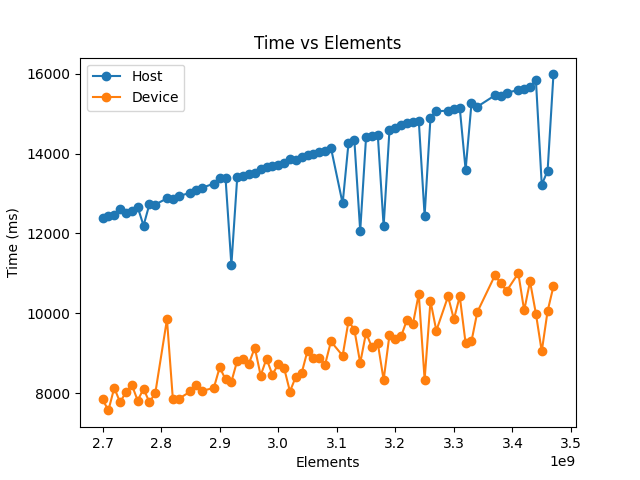
\includegraphics[width=0.9\textwidth]{./imagenes/P2_1/time_vs_elements.png}
				}
				\caption{Tiempo de ejecución en función del número de elementos.}
				\label{fig:time_vs_elements_1}
			\end{figure}

			\begin{figure}
				\centering
				\fbox{
					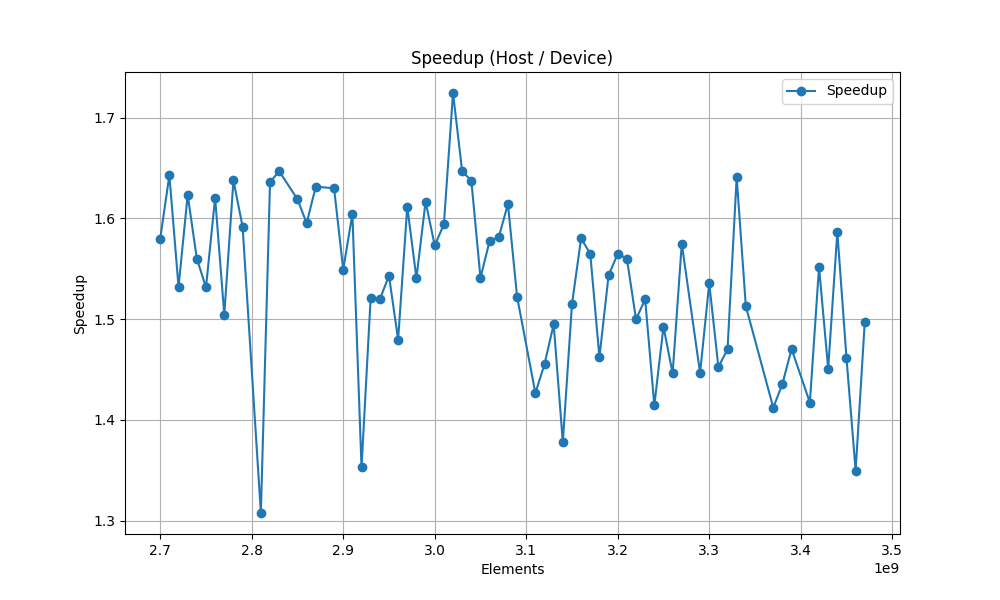
\includegraphics[width=0.9\textwidth]{./imagenes/P2_1/speedup.png}
				}
				\caption{\textit{Speedup} en función del número de elementos.}
				\label{fig:speedup_1}
			\end{figure}

		\subsubsection{Análisis de resultados}

			En este apartado se analiza el rendimiento de la suma de vectores en la CPU (\textit{host}) y la GPU (\textit{device}), integrando los datos obtenidos y las visualizaciones proporcionadas en las Figuras \ref{fig:time_vs_elements_1} y \ref{fig:speedup_1}. Se evalúa el comportamiento de los tiempos de ejecución, la escalabilidad, y el \textit{speedup} logrado en función del tamaño de los vectores.

			La Figura \ref{fig:time_vs_elements_1} muestra los tiempos de ejecución en función del número de elementos en los vectores para la CPU y la GPU. Como se observa, el tiempo de la CPU crece de forma casi lineal con el tamaño de los vectores, lo cual es consistente con el hecho de que cada elemento se procesa secuencialmente. Por el contrario, en la GPU, el tiempo presenta fluctuaciones menores pero sigue una tendencia general de incremento con el tamaño de los vectores. Esto se debe a que, si bien la GPU puede procesar miles de elementos en paralelo, la sobrecarga asociada a la gestión de la memoria y la comunicación entre \textit{host} y \textit{device} introduce cierta variabilidad.

			Es importante notar que, a medida que se incrementa el tamaño de los vectores, la GPU mantiene un rendimiento significativamente mejor que la CPU. Sin embargo, los tiempos de la GPU no son completamente lineales, lo cual puede atribuirse a limitaciones del \textit{hardware}, como la saturación de los recursos de memoria global o la cantidad limitada de multiprocesadores disponibles para un número muy elevado de bloques.

			La Figura \ref{fig:speedup_1} representa el \textit{speedup} (\textit{Host/Device}) en función del tamaño de los vectores. En términos generales, se observa que el \textit{speedup} se mantiene consistentemente por encima de 1, lo que confirma que la GPU ofrece una aceleración significativa en comparación con la CPU.

			Estas variaciones en el \textit{speedup} pueden explicarse por la influencia de factores como la alineación de los datos en memoria, la eficiencia en la asignación de \textit{threads} por bloque y la sobrecarga de la transferencia de datos. Cuando los datos se distribuyen de forma óptima y las transferencias de memoria son mínimas en comparación con el cómputo, se logran los valores de \textit{speedup} más altos. Por otro lado, en casos donde las transferencias de memoria tienen un impacto mayor, el \textit{speedup} disminuye.

			Los resultados indican que el rendimiento en la GPU es altamente escalable para tamaños de vectores grandes. Sin embargo, se identifican ciertos puntos donde el tiempo de la GPU aumenta de manera más significativa. Esto sugiere que, a partir de cierto umbral, las transferencias de memoria y la saturación de los recursos del dispositivo comienzan a impactar de manera más visible en el tiempo total de ejecución. A pesar de estas limitaciones, la GPU sigue siendo más eficiente que la CPU para todos los tamaños de vectores evaluados. Esto demuestra la capacidad de la GPU para manejar grandes volúmenes de datos de manera paralela, aprovechando su arquitectura masivamente paralela.

			De acuerdo con los datos y las visualizaciones presentadas, se puede concluir que:

			\begin{itemize}

				\item El tiempo en la CPU crece de manera lineal con el tamaño de los vectores, mientras que en la GPU se observan fluctuaciones debido a factores de \textit{hardware} y memoria.

				\item El \textit{speedup} logrado por la GPU es consistente y significativo, alcanzando un máximo de 2.6, con valores promedio cercanos a 1.8.

				\item La GPU demuestra una mejor escalabilidad y capacidad de procesamiento paralelo, lo que la hace más adecuada para aplicaciones que involucren grandes volúmenes de datos.

			\end{itemize}

	\subsection{Apartado 2}

		\subsubsection{Resultados obtenidos}

			En este apartado se midió el tiempo de ejecución del código \texttt{vectorAdd.cu} para un vector de tamaño fijo, tamaño 3480000000, utilizando una GPU A100 y variando el número de \textit{threads} por bloque. Los resultados obtenidos se presentan en la Tabla \ref{tab:resultados2} y las Figuras \ref{fig:threads_vs_time_2} y \ref{fig:threads_vs_blocks_2}.

			\begin{table}[H]
				\centering
				\begin{adjustbox}{width=\textwidth, keepaspectratio}
					\begin{tabular}{|r|r|r|r|r|r|}
						\hline
						elements & blocks & threads & repts & time\_host & time\_dev \\ \hline
						3480000000 & 108750000 & 32 & 1 & 14773.328 & 10207.448 \\ \hline
						3480000000 & 54375000 & 64 & 1 & 14466.421 & 6622.943 \\ \hline
						3480000000 & 36250000 & 96 & 1 & 14982.508 & 9829.690 \\ \hline
						3480000000 & 27187500 & 128 & 1 & 14615.394 & 10038.033 \\ \hline
						3480000000 & 21750000 & 160 & 1 & 14651.510 & 10364.214 \\ \hline
						3480000000 & 18125000 & 192 & 1 & 14594.880 & 10118.989 \\ \hline
						3480000000 & 15535715 & 224 & 1 & 14606.531 & 10009.701 \\ \hline
						3480000000 & 13593750 & 256 & 1 & 14488.415 & 9917.299 \\ \hline
						3480000000 & 12083334 & 288 & 1 & 14566.970 & 9637.912 \\ \hline
						3480000000 & 10875000 & 320 & 1 & 14594.865 & 9913.020 \\ \hline
						3480000000 & 9886364 & 352 & 1 & 14577.759 & 9884.579 \\ \hline
						3480000000 & 9062500 & 384 & 1 & 14592.525 & 10041.159 \\ \hline
						3480000000 & 8365385 & 416 & 1 & 14569.258 & 9648.561 \\ \hline
						3480000000 & 7767858 & 448 & 1 & 14589.233 & 9746.657 \\ \hline
						3480000000 & 7250000 & 480 & 1 & 14946.919 & 9917.020 \\ \hline
						3480000000 & 6796875 & 512 & 1 & 14987.132 & 9944.101 \\ \hline
						3480000000 & 6397059 & 544 & 1 & 14938.825 & 9522.819 \\ \hline
						3480000000 & 6041667 & 576 & 1 & 14584.061 & 9789.817 \\ \hline
						3480000000 & 5723685 & 608 & 1 & 14566.116 & 10072.887 \\ \hline
						3480000000 & 5437500 & 640 & 1 & 14599.345 & 10024.539 \\ \hline
						3480000000 & 5178572 & 672 & 1 & 14606.157 & 6445.615 \\ \hline
						3480000000 & 4943182 & 704 & 1 & 14567.088 & 9731.308 \\ \hline
						3480000000 & 4728261 & 736 & 1 & 13311.289 & 6750.650 \\ \hline
						3480000000 & 4531250 & 768 & 1 & 14621.899 & 10388.275 \\ \hline
						3480000000 & 4350000 & 800 & 1 & 14553.650 & 9666.851 \\ \hline
						3480000000 & 4182693 & 832 & 1 & 14588.173 & 10073.638 \\ \hline
						3480000000 & 4027778 & 864 & 1 & 14597.753 & 10068.537 \\ \hline
						3480000000 & 3883929 & 896 & 1 & 13344.991 & 6282.809 \\ \hline
						3480000000 & 3750000 & 928 & 1 & 14558.886 & 9865.713 \\ \hline
						3480000000 & 3625000 & 960 & 1 & 14615.697 & 10038.352 \\ \hline
						3480000000 & 3508065 & 992 & 1 & 14559.104 & 10048.968 \\ \hline \hline
						3480000000 & 3398438 & 1024 & 1 & 14554.076 & 10025.835 \\ \hline
					\end{tabular}
				\end{adjustbox}
				\caption{Tiempos de ejecución para diferentes valores de threads.}
				\label{tab:resultados2}
			\end{table}

			\begin{figure}[H]
				\centering
				\fbox{
					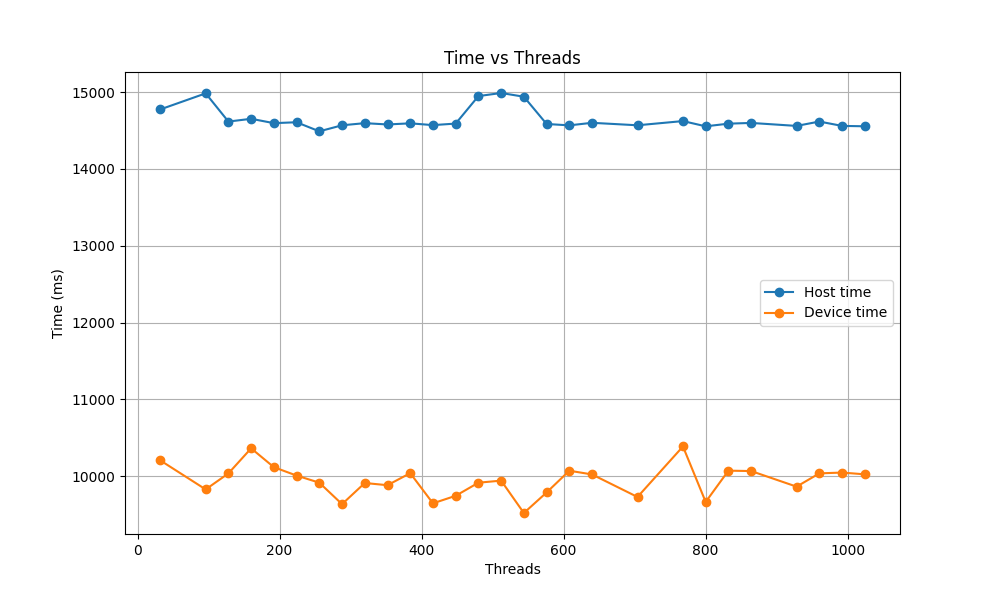
\includegraphics[width=0.9\textwidth]{./imagenes/P2_2/threads_vs_time.png}
				}
				\caption{Tiempo de ejecución en función del número de \textit{threads}.}
				\label{fig:threads_vs_time_2}
			\end{figure}

			\begin{figure}
				\centering
				\fbox{
					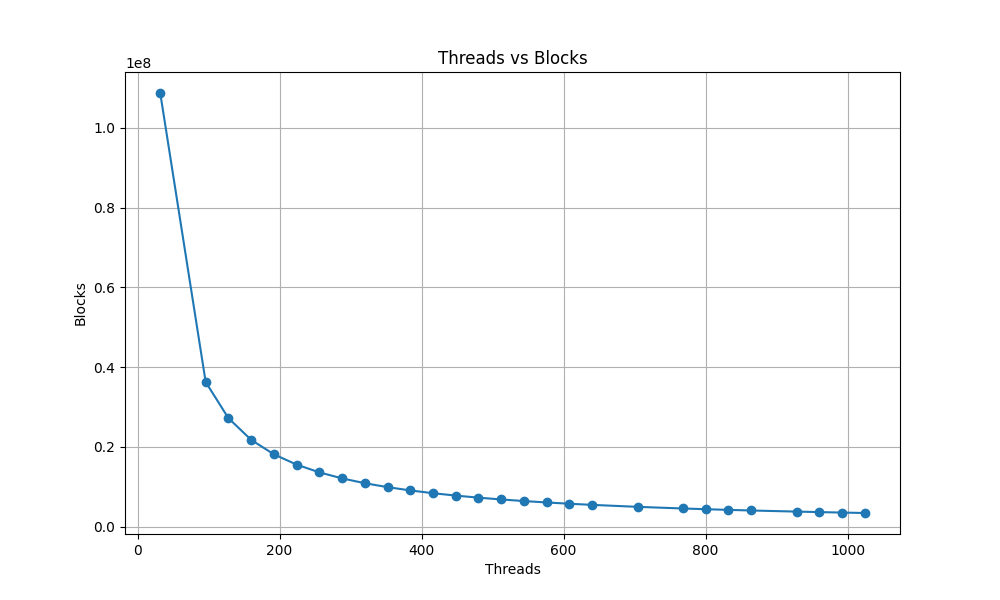
\includegraphics[width=0.9\textwidth]{./imagenes/P2_2/threads_vs_blocks.png}
				}
				\caption{Número de bloques en función del número de \textit{threads}.}
				\label{fig:threads_vs_blocks_2}
			\end{figure}

		\subsubsection{Análisis de resultados}

			En este apartado se analizan los datos obtenidos de la ejecución del programa para la suma de vectores en CPU y GPU, considerando configuraciones con diferentes cantidades de hilos y bloques. Se presentan los resultados en función del rendimiento en términos de tiempos de ejecución y se discuten las implicaciones del escalado en el número de hilos y bloques. Para ello, se analizan las Figuras \ref{fig:threads_vs_blocks_2} y \ref{fig:threads_vs_time_2}, así como la tabla de datos recopilados, con el objetivo de comprender cómo la configuración de hilos y bloques afecta el rendimiento de la GPU.

			La Figura \ref{fig:threads_vs_blocks_2} ilustra la relación inversa entre el número de hilos por bloque y el número de bloques necesarios para procesar un tamaño fijo de datos (en este caso, 3,48 mil millones de elementos). A medida que aumenta el número de hilos por bloque, el número de bloques disminuye de forma drástica. Esto es consistente con el diseño de las GPUs, donde el trabajo se distribuye en múltiples hilos que procesan en paralelo. Una mayor cantidad de hilos por bloque reduce la necesidad de bloques adicionales, optimizando el uso de los recursos del \textit{hardware}.

			Sin embargo, hay un límite en el número de hilos por bloque impuesto por la arquitectura de la GPU. Este límite condiciona las configuraciones posibles y puede influir en el rendimiento general, especialmente en problemas donde el tamaño de los datos no es perfectamente divisible por el producto de bloques e hilos.

			En la Figura \ref{fig:threads_vs_time_2}, se examinan los tiempos de ejecución en la CPU y GPU para diferentes configuraciones de hilos, manteniendo constante el tamaño del vector. En la CPU, los tiempos permanecen relativamente constantes, ya que no depende directamente del número de hilos de la GPU. En contraste, en la GPU se observa una fluctuación en los tiempos de ejecución, lo que refleja cómo la configuración de bloques e hilos afecta el rendimiento.

			Para configuraciones de 286 y 544 hilos por bloque, se alcanzan tiempos significativamente más bajos. Esto sugiere que estas configuraciones representan un balance óptimo entre el número de hilos por bloque y la sobrecarga asociada a la administración de recursos. Sin embargo, en configuraciones con números de hilos intermedios o cercanos a los extremos del rango evaluado, los tiempos tienden a aumentar debido a una menor eficiencia en la asignación de recursos o a un mayor \textit{overhead}.

			Los datos muestran que la GPU sigue siendo significativamente más rápida que la CPU en todas las configuraciones de hilos evaluadas, con un tiempo promedio de la GPU oscilando entre 6 y 10 segundos, mientras que el tiempo en la CPU se mantiene alrededor de 14.5 segundos. Este resultado pone de manifiesto la ventaja inherente de las GPUs en tareas paralelas, aunque también resalta la importancia de seleccionar configuraciones adecuadas para maximizar el rendimiento.

			Adicionalmente, se observa que el rendimiento de la GPU no es uniforme en todas las configuraciones. Las fluctuaciones reflejan las interacciones complejas entre las transferencias de memoria, la cantidad de bloques y la cantidad de hilos por bloque. Configuraciones subóptimas, donde los recursos no se utilizan plenamente, pueden dar lugar a mayores tiempos de ejecución.

			De acuerdo con los datos presentados y las visualizaciones en las Figuras \ref{fig:threads_vs_blocks_2} y \ref{fig:threads_vs_time_2}, se concluye lo siguiente:

			\begin{itemize}

				\item La relación entre hilos y bloques sigue una tendencia inversa. Configuraciones con un mayor número de hilos por bloque requieren menos bloques, optimizando el paralelismo.

				\item La GPU supera consistentemente a la CPU en tiempos de ejecución, aunque el rendimiento de la GPU varía con la configuración de hilos y bloques.

				\item Las configuraciones de 286 y 544 hilos por bloque parecen ofrecer el mejor rendimiento, destacándose como puntos óptimos en el balance entre hilos, bloques y \textit{overhead}.

				\item Los tiempos en la GPU son sensibles a configuraciones subóptimas, lo que resalta la importancia de comprender las limitaciones arquitectónicas al diseñar aplicaciones paralelas.

			\end{itemize}

	\subsection{Apartado 3}

		\subsubsection{Resultados obtenidos}

			En este apartado se midió el tiempo de ejecución del código \texttt{vectorAdd.cu} para un vector de tamaño fijo, tamaño 3480000000, utilizando una GPU A100, manteniendo constantes los valores de número de bloques e hilos pero variando el número de repeticiones del lazo. Los resultados obtenidos se presentan en la Tabla \ref{tab:resultados3} y las Figuras \ref{fig:repts_vs_time_3} y \ref{fig:speedup_vs_repts_3}.

			\begin{table}[H]
				\begin{adjustbox}{width=\textwidth, keepaspectratio}
					\begin{tabular}{|r|r|r|r|r|r|}
						\hline
						elements & blocks & threads & repts & time\_host & time\_dev \\ \hline
						3480000000 & 6397059 & 544 & 1 & 15929.340 & 16674.916 \\ \hline
						3480000000 & 6397059 & 544 & 2 & 26827.312 & 9962.560 \\ \hline
						3480000000 & 6397059 & 544 & 3 & 37525.497 & 9680.245 \\ \hline
						3480000000 & 6397059 & 544 & 4 & 51515.259 & 10008.560 \\ \hline
						3480000000 & 6397059 & 544 & 5 & 63471.979 & 10108.948 \\ \hline
						3480000000 & 6397059 & 544 & 6 & 74938.242 & 10114.232 \\ \hline
						3480000000 & 6397059 & 544 & 7 & 87200.833 & 9813.671 \\ \hline
						3480000000 & 6397059 & 544 & 8 & 99132.063 & 9964.844 \\ \hline
						3480000000 & 6397059 & 544 & 9 & 110922.887 & 10359.982 \\ \hline
						3480000000 & 6397059 & 544 & 10 & 122735.950 & 9955.548 \\ \hline
						3480000000 & 6397059 & 544 & 11 & 134802.104 & 10211.383 \\ \hline
						3480000000 & 6397059 & 544 & 12 & 146549.000 & 10031.169 \\ \hline
						3480000000 & 6397059 & 544 & 13 & 158659.116 & 6152.381 \\ \hline
						3480000000 & 6397059 & 544 & 14 & 170649.806 & 6344.022 \\ \hline
						3480000000 & 6397059 & 544 & 15 & 179044.220 & 9846.553 \\ \hline
						3480000000 & 6397059 & 544 & 16 & 194031.500 & 10608.078 \\ \hline
						3480000000 & 6397059 & 544 & 17 & 205995.775 & 7392.401 \\ \hline
						3480000000 & 6397059 & 544 & 18 & 215657.783 & 6762.759 \\ \hline
						3480000000 & 6397059 & 544 & 19 & 229825.838 & 10423.736 \\ \hline
						3480000000 & 6397059 & 544 & 20 & 241822.356 & 10375.769 \\ \hline
						3480000000 & 6397059 & 544 & 21 & 250648.282 & 6513.722 \\ \hline
						3480000000 & 6397059 & 544 & 22 & 265605.998 & 6663.431 \\ \hline
						3480000000 & 6397059 & 544 & 23 & 275205.110 & 6465.822 \\ \hline
						3480000000 & 6397059 & 544 & 24 & 289067.561 & 10317.736 \\ \hline
						3480000000 & 6397059 & 544 & 25 & 301374.468 & 10747.888 \\ \hline
						3480000000 & 6397059 & 544 & 26 & 313087.429 & 10483.567 \\ \hline
						3480000000 & 6397059 & 544 & 27 & 323979.058 & 10195.237 \\ \hline
						3480000000 & 6397059 & 544 & 28 & 337238.283 & 10654.639 \\ \hline
					\end{tabular}
				\end{adjustbox}
				\caption{Tiempos de ejecución para diferentes valores de repeticiones.}
				\label{tab:resultados3}
			\end{table}

			\begin{figure}
				\centering
				\fbox{
					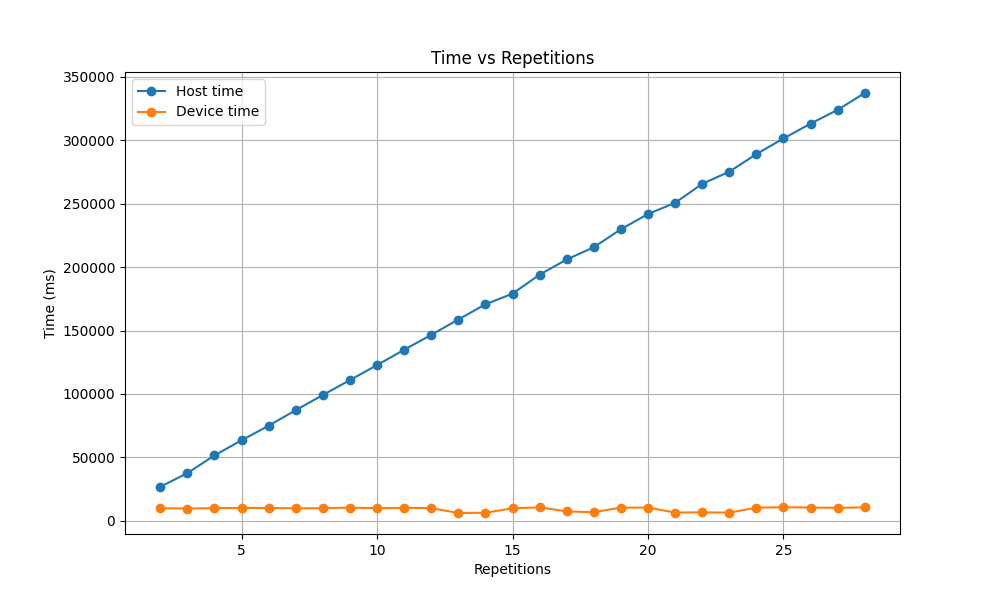
\includegraphics[width=0.9\textwidth]{./imagenes/P2_3/time_vs_repts.png}
				}
				\caption{Tiempo de ejecución en función del número de repeticiones.}
				\label{fig:repts_vs_time_3}
			\end{figure}

			\begin{figure}
				\centering
				\fbox{
					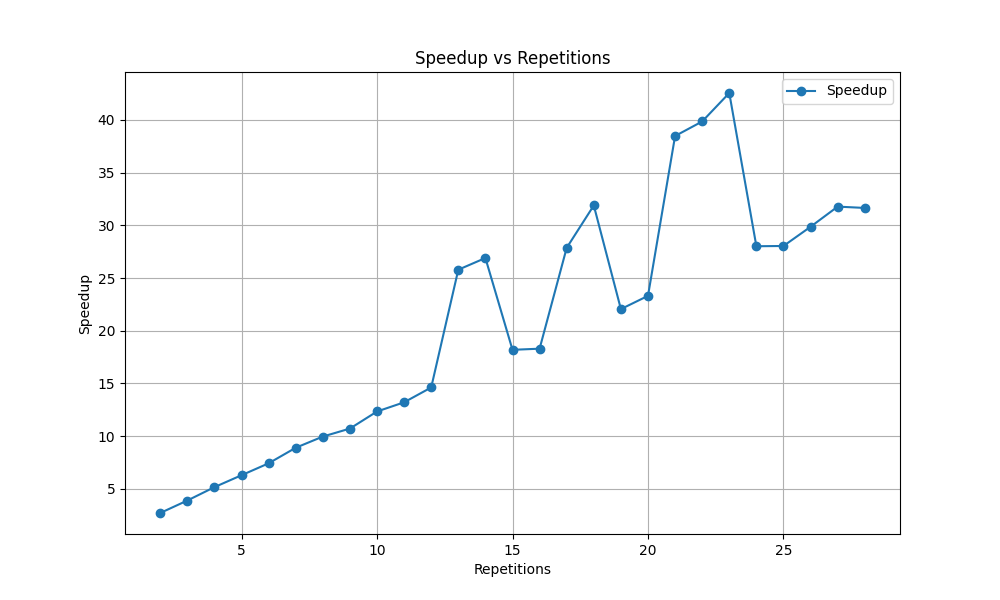
\includegraphics[width=0.9\textwidth]{./imagenes/P2_3/speedup_vs_repts.png}
				}
				\caption{\textit{Speedup} en función del número de repeticiones.}
				\label{fig:speedup_vs_repts_3}
			\end{figure}

		\subsubsection{Análisis de resultados}

			En este apartado se analizan los resultados obtenidos al variar el número de repeticiones (\texttt{repts}) del cálculo sumatorio entre dos vectores. Se evalúa cómo esta variación influye en los tiempos de ejecución tanto en la CPU como en la GPU, además de observar el comportamiento del \textit{speedup} en función del número de repeticiones.

			La Tabla \ref{tab:resultados3} presenta los tiempos de ejecución en la CPU (\texttt{time\_host}) y en la GPU (\texttt{time\_dev}) para diferentes valores de repeticiones, manteniendo constantes el número de bloques (6397059) y los hilos por bloque (544). Estos parámetros corresponden a configuraciones óptimas determinadas en experimentos previos para el \textit{hardware} utilizado. Como se observa, los tiempos de la CPU aumentan progresivamente con el número de repeticiones, siguiendo una tendencia lineal. Este incremento se debe a la arquitectura secuencial de la CPU, que limita su rendimiento en tareas altamente paralelizables. A medida que se incrementan las repeticiones, el conjunto de instrucciones debe ejecutarse más veces, lo que deriva en un aumento lineal del tiempo de ejecución.

			En contraste, los tiempos de ejecución en la GPU muestran un comportamiento diferente. Aunque también incrementan con el número de repeticiones, este aumento es mucho menor en comparación con la CPU. Los resultados indican que la variación del tiempo en la GPU es mínima, lo que sugiere que el tiempo de cómputo en la GPU no es el factor limitante. En su lugar, parece que la transferencia de datos entre el \textit{host} (CPU) y el dispositivo (GPU) es el principal cuello de botella. El impacto de este costo de transferencia se reduce a medida que se amortigua con un mayor número de cálculos paralelizados, lo que resulta en tiempos de ejecución casi constantes para la GPU.

			La Figura \ref{fig:speedup_vs_repts_3} muestra la relación entre los tiempos de ejecución de la CPU y la GPU (\textit{speedup}) en función del número de repeticiones. En general, el \textit{speedup} mejora de manera lineal a medida que aumentan las repeticiones. Este comportamiento indica que la GPU aprovecha su arquitectura masivamente paralela de forma más eficiente a medida que se incrementa la carga de trabajo. Además, refleja cómo el costo de transferencia de datos se diluye en un mayor número de cálculos, optimizando el rendimiento relativo de la GPU.

			Finalmente, la Figura \ref{fig:repts_vs_time_3} ilustra, al igual que la Tabla \ref{tab:resultados3}, cómo los tiempos de ejecución en la CPU aumentan linealmente con el número de repeticiones, mientras que en la GPU permanecen relativamente constantes. Este resultado pone de manifiesto la alta eficiencia de la GPU en tareas paralelizables y la importancia de considerar la sobrecarga de transferencia de datos al diseñar aplicaciones para este tipo de \textit{hardware}. En conclusión, los resultados demuestran que la GPU es significativamente más eficiente que la CPU en cálculos repetitivos, siempre y cuando se minimice la sobrecarga asociada a la transferencia de datos, maximizando así el rendimiento global.

			Basado en los resultados presentados en la Tabla \ref{tab:resultados3} y las gráficas \ref{fig:repts_vs_time_3} y \ref{fig:speedup_vs_repts_3}, se pueden hacer las siguientes observaciones:

			\begin{itemize}

				\item Los tiempos de ejecución en la CPU aumentan de manera lineal con el número de repeticiones, mientras que en la GPU se mantienen relativamente constantes.

				\item La GPU se beneficia de la ejecución paralela al realizar múltiples repeticiones, lo que se refleja en un \textit{speedup} creciente con el número de repeticiones.

				\item La transferencia de datos entre la CPU y la GPU es un factor crítico en el rendimiento, y amortiguar este costo en un mayor número de cálculos paralelizados puede mejorar significativamente el rendimiento total.

				\item La GPU es más eficiente en tareas repetitivas, pero es importante minimizar la sobrecarga de la transferencia de datos para optimizar el rendimiento.

			\end{itemize}

	\subsection{Apartado 4}

		\subsubsection{Resultados obtenidos}

			En este apartado se midió el tiempo de ejecución del código \texttt{vectorAdd.cu} variando el tamaño del vector y manteniendo constantes los valores de número de bloques e hilos por bloque. A diferencia de apartados anteriores en este se realizaron modificaciones al código original para permitir obtener los valores de tiempo para distintos puntos clave del programa como el tiempo de ejecución en la CPU (\textit{Host}), el tiempo de ejecución en la GPU (\textit{Device}) y los tiempos de transferencia de datos entre el \textit{Host} y la GPU entre otros. Los resultados obtenidos se presentan en la Tablas \ref{tab:resultados4_1}, \ref{tab:resultados4_2} y \ref{tab:resultados4_3} así como las Figuras \ref{fig:time_breakdown_4}, \ref{fig:device_vs_host_time_4} y \ref{fig:speedup_vs_elements_4}. Gracias a estas modificaciones se busca obtener una mejor comprensión del rendimiento del programa y de los factores clave que influyen en el tiempo de ejecución.

			\begin{table}[H]
				\begin{adjustbox}{width=\textwidth, height=\textheight, keepaspectratio}
					\begin{tabular}{|r|r|r|r|r|r|r|r|r|}
						\hline
						elements & blocks & threads & repts & time\_host & time\_dev\_malloc & time\_host\_to\_dev & time\_dev\_kernel & time\_dev\_to\_host \\ \hline
						2600000000 & 10156250 & 256 & 1 & 9900.670 & 555.954 & 1955.851 & 22.803 & 4602.516 \\ \hline
						2700000000 & 10546875 & 256 & 1 & 10328.920 & 215.466 & 1827.690 & 23.691 & 2466.349 \\ \hline
						2800000000 & 10937500 & 256 & 1 & 10691.320 & 670.005 & 2095.931 & 24.527 & 5505.592 \\ \hline
						2900000000 & 11328125 & 256 & 1 & 11120.870 & 228.032 & 2061.650 & 25.399 & 4585.718 \\ \hline
						3000000000 & 11718750 & 256 & 1 & 11398.130 & 678.784 & 1997.767 & 26.292 & 2744.937 \\ \hline
						3100000000 & 12109375 & 256 & 1 & 12668.800 & 239.777 & 2330.564 & 27.163 & 6127.359 \\ \hline
						3200000000 & 12500000 & 256 & 1 & 13170.600 & 666.078 & 2319.245 & 28.014 & 6347.536 \\ \hline
						3300000000 & 12890625 & 256 & 1 & 13762.810 & 661.145 & 2370.431 & 28.927 & 6497.531 \\ \hline
						3400000000 & 13281250 & 256 & 1 & 14473.660 & 558.613 & 2596.730 & 29.792 & 7042.505 \\ \hline
						3480000000 & 13593750 & 256 & 1 & 14838.280 & 257.880 & 2595.574 & 30.472 & 7129.856 \\ \hline
					\end{tabular}
				\end{adjustbox}
				\caption{Tiempos de ejecución para diferentes valores de número de elementos.}
				\label{tab:resultados4_1}
			\end{table}

			\begin{table}[H]
				\begin{adjustbox}{width=\textwidth, height=\textheight, keepaspectratio}
					\begin{tabular}{|r|r|r|r|r|r|}
						\hline
						elements & total\_time & \%\_time\_dev\_malloc & \%\_time\_host\_to\_dev & \%\_time\_dev\_kernel & \%\_time\_dev\_to\_host \\ \hline
						2600000000 & 7137.124 & 7.79 & 27.40 & 0.32 & 64.49 \\ \hline
						2700000000 & 4533.196 & 4.75 & 40.32 & 0.52 & 54.41 \\ \hline
						2800000000 & 8296.055 & 8.08 & 25.26 & 0.30 & 66.36 \\ \hline
						2900000000 & 6900.799 & 3.30 & 29.88 & 0.37 & 66.45 \\ \hline
						3000000000 & 5447.780 & 12.46 & 36.67 & 0.48 & 50.39 \\ \hline
						3100000000 & 8724.863 & 2.75 & 26.71 & 0.31 & 70.23 \\ \hline
						3200000000 & 9360.873 & 7.12 & 24.78 & 0.30 & 67.81 \\ \hline
						3300000000 & 9558.034 & 6.92 & 24.80 & 0.30 & 67.98 \\ \hline
						3400000000 & 10227.640 & 5.46 & 25.39 & 0.29 & 68.86 \\ \hline
						3480000000 & 10013.782 & 2.58 & 25.92 & 0.30 & 71.20 \\ \hline
					\end{tabular}
				\end{adjustbox}
				\caption{Desglose del tiempo de ejecución en diferentes fases para diferentes valores de número de elementos.}
				\label{tab:resultados4_2}
			\end{table}

			\begin{table}[H]
				\begin{adjustbox}{width=\textwidth, keepaspectratio}
					\begin{tabular}{|r|r|r|r|} \hline
						elements & time\_host & time\_dev\_kernel & \%\_improvement \\ \hline
						2600000000 & 9900.670 & 22.803 & 43318.28 \\ \hline
						2700000000 & 10328.920 & 23.691 & 43498.50 \\ \hline
						2800000000 & 10691.320 & 24.527 & 43490.00 \\ \hline
						2900000000 & 11120.870 & 25.399 & 43684.68 \\ \hline
						3000000000 & 11398.130 & 26.292 & 43252.08 \\ \hline
						3100000000 & 12668.800 & 27.163 & 46539.91 \\ \hline
						3200000000 & 13170.600 & 28.014 & 46914.35 \\ \hline
						3300000000 & 13762.810 & 28.927 & 47477.73 \\ \hline
						3400000000 & 14473.660 & 29.792 & 48482.37 \\ \hline
						3480000000 & 14838.280 & 30.472 & 48594.80 \\ \hline
					\end{tabular}
				\end{adjustbox}
				\caption{Diferencia de tiempo de ejecución real entre el \textit{host} y el \textit{device} para diferentes valores de número de elementos.}
				\label{tab:resultados4_3}
			\end{table}

			\begin{figure}
				\centering
				\fbox{
					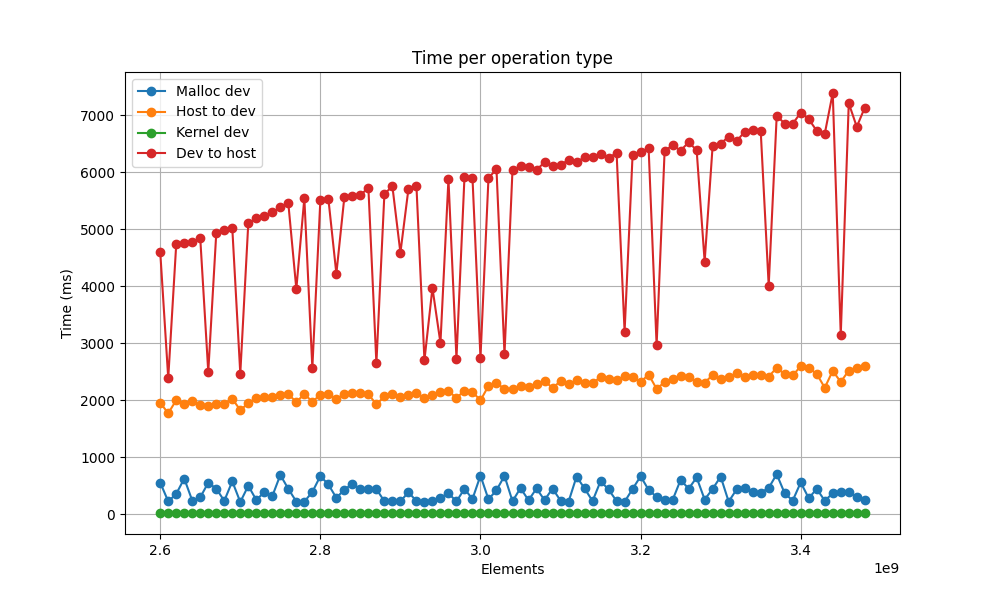
\includegraphics[width=0.9\textwidth]{./imagenes/P2_4/time_per_operation_type.png}
				}
				\caption{Desglose del tiempo de ejecución en diferentes fases.}
				\label{fig:time_breakdown_4}
			\end{figure}

			\begin{figure}
				\centering
				\fbox{
					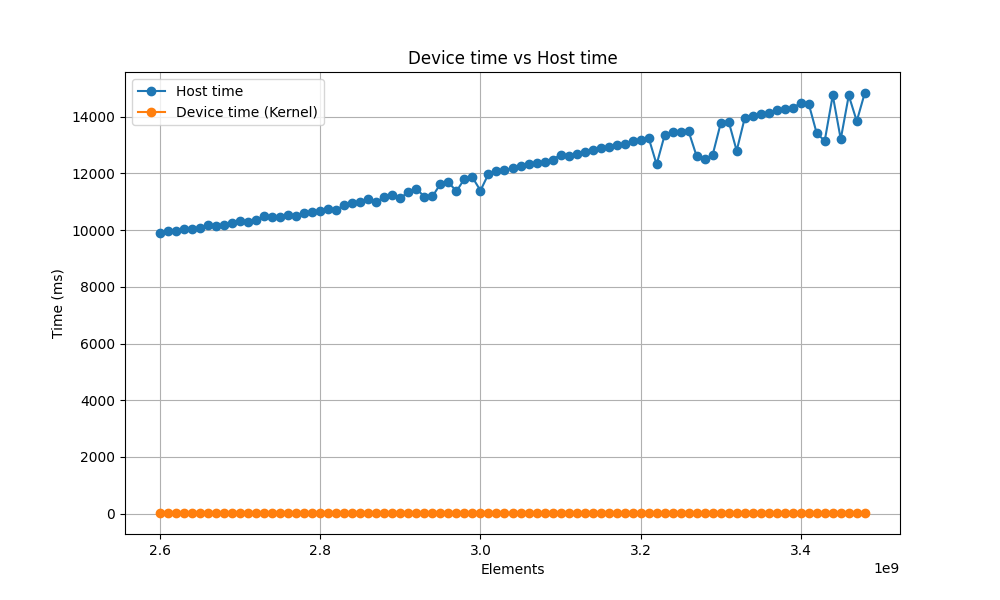
\includegraphics[width=0.9\textwidth]{./imagenes/P2_4/device_vs_host_time.png}
				}
				\caption{Tiempo de ejecución real en el \textit{host} y el \textit{device}.}
				\label{fig:device_vs_host_time_4}
			\end{figure}

			\begin{figure}
				\centering
				\fbox{
					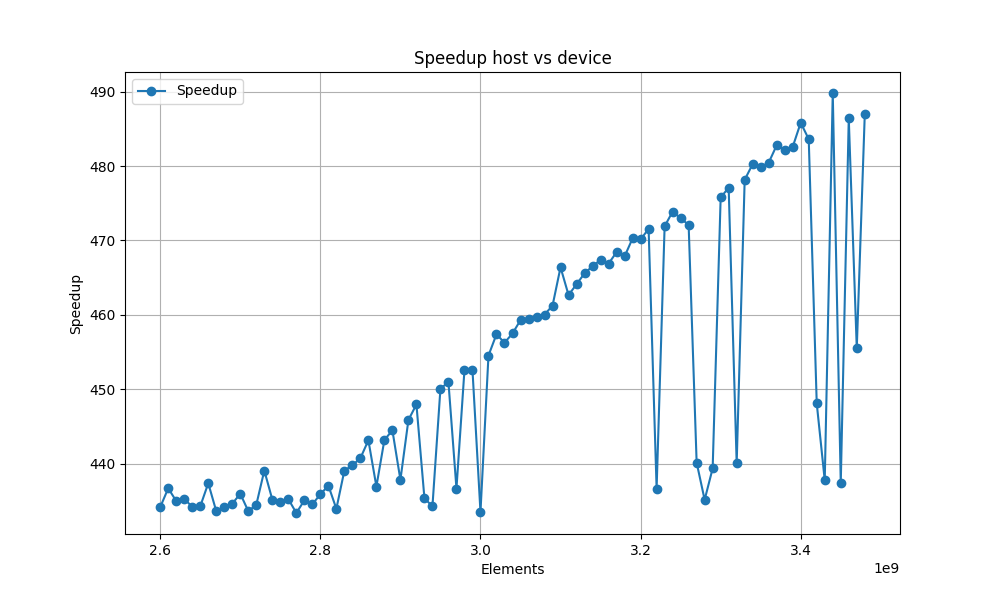
\includegraphics[width=0.9\textwidth]{./imagenes/P2_4/speedup_vs_elements.png}
				}
				\caption{\textit{Speedup} real en función del número de elementos.}
				\label{fig:speedup_vs_elements_4}
			\end{figure}

		\subsubsection{Análisis de resultados}

			En este apartado se presenta un análisis detallado de los tiempos de ejecución obtenidos, desglosando el tiempo total según las diferentes fases del proceso. Las fases consideradas en este análisis incluyen la ejecución del cálculo en el \textit{host}, la reserva de memoria en la GPU (\textit{device}), las transferencias de datos entre el \textit{host} y el dispositivo, la ejecución del \textit{kernel} en el dispositivo, y la transferencia de datos de vuelta al \textit{host}. El objetivo principal de este análisis es identificar las fases que consumen más tiempo, con el fin de entender mejor el comportamiento del algoritmo y poder identificar posibles áreas de mejora.

			En las tablas anteriores se presenta el tiempo total de ejecución y el porcentaje de tiempo consumido por cada fase, considerando diferentes valores de elementos procesados. De forma complementaria, la figura \ref{fig:time_breakdown_4} ilustra gráficamente el desglose temporal de las distintas fases. A partir de estos resultados, se observa que las fases que más tiempo consumen son la transferencia de datos de vuelta al \textit{host} y la transferencia de datos entre el \textit{host} y el dispositivo. En contraposición, la ejecución del \textit{kernel} en el dispositivo resulta ser la fase con menor tiempo de ejecución. Estos resultados concuerdan con lo esperado, dado que las transferencias de datos son operaciones de entrada y salida, las cuales suelen ser significativamente más costosas en términos de tiempo en comparación con las operaciones de cómputo realizadas en el dispositivo. Además, los resultados obtenidos son consistentes con los datos analizados en secciones anteriores del estudio.

			En las otras tablas se muestra la diferencia de tiempo de ejecución al comparar exclusivamente la ejecución del \textit{kernel} entre el \textit{host} y el dispositivo. Esta diferencia se representa también gráficamente en la figura \ref{fig:device_vs_host_time_4}. Los resultados muestran que el tiempo de ejecución en el dispositivo siempre es inferior al tiempo de ejecución en el \textit{host}. Además, la diferencia entre ambos tiempos aumenta conforme lo hace el número de elementos procesados. Este comportamiento se debe a que el tiempo de ejecución en el \textit{host} crece de manera aproximadamente lineal con el número de elementos, mientras que el tiempo de ejecución en el dispositivo permanece relativamente constante, independientemente del tamaño de los datos gracias a la capacidad de paralelización de la GPU. Del mismo modo podemos observar cómo los tiempo consumidos para los cálculos en el dispositivo son significativamente menores que los tiempos consumidos en el \textit{host}, lo que se traduce en un \textit{speedup} que aumenta conforme aumenta el número de elementos, lo que evidencia una mayor eficiencia del dispositivo en comparación con el \textit{host} al procesar grandes volúmenes de datos y su idoneidad para tareas computacionales intensivas.

			Por otro lado, la figura \ref{fig:speedup_vs_elements_4} muestra el \textit{speedup} en función del número de elementos procesados. En este gráfico se observa que el \textit{speedup} aumenta conforme aumenta el número de elementos, lo que evidencia una mayor eficiencia del dispositivo en comparación con el \textit{host} al procesar grandes volúmenes de datos. En esta gráfica se observa como el \textit{speedup} obtenido es mayor para los casos en los que se procesan un mayor número de elementos, lo que indica que la GPU es más eficiente para manejar grandes volúmenes de datos. Por otro lado, el \textit{speedup} obtenido es menor para los casos en los que se procesan un menor número de elementos, lo que indica que la GPU es menos eficiente para manejar pequeños volúmenes de datos. En general, los resultados obtenidos son consistentes con las expectativas previas y confirman la ventaja de la GPU para tareas computacionales intensivas, aunque el tiempo de transferencia de datos sigue siendo un área por optimizar.

			A partir de los resultados obtenidos, se pueden derivar las siguientes conclusiones:

			\begin{itemize}

				\item El uso de la GPU para la ejecución del algoritmos altamente paralelizables es más eficiente que el uso de la CPU, ya que el tiempo de ejecución en el dispositivo es menor que en el \textit{host}.

				\item El \textit{speedup} es mayor conforme aumenta el número de elementos, lo que demuestra que la GPU es más eficiente para manejar grandes volúmenes de datos.

				\item Las fases que consumen más tiempo son la transferencia de datos entre el \textit{host} y el dispositivo, así como la transferencia de datos de vuelta al \textit{host}. Estas son operaciones costosas debido a su naturaleza de entrada/salida.

				\item La ejecución del \textit{kernel} en el dispositivo es la fase que menos tiempo consume, lo que resalta la eficiencia del procesamiento en la GPU.

				\item La diferencia de tiempo de ejecución entre el \textit{host} y el dispositivo aumenta con el número de elementos, lo que se debe a que el tiempo de ejecución en el \textit{host} crece de manera lineal mientras que el tiempo de ejecución en el dispositivo se mantiene casi constante.

				\item Los resultados son consistentes con las expectativas previas y confirman la ventaja de la GPU para tareas computacionales intensivas, aunque el tiempo de transferencia de datos sigue siendo un área por optimizar.

			\end{itemize}

	\subsection{Apartado 5}

		\subsubsection{Resultados obtenidos}

			En este apartado se presenta un análisis del rendimiento del algoritmo implementado en el apartado anterior, considerando una mejora en la gestión de la memoria. En concreto, se ha modificado el código original para utilizar memoria unificada, lo que permite al programador trabajar con un espacio de memoria único que es accesible tanto desde el \textit{host} como desde el dispositivo. De esta forma, se evita la necesidad de transferir datos entre el \textit{host} y el dispositivo de forma explícita por el programador, lo que puede resultar en una mejora significativa del rendimiento. El objetivo de este análisis es evaluar el impacto de esta mejora en el rendimiento del algoritmo y compararlo con la solución original.

			\begin{figure}
				\centering
				\fbox{
					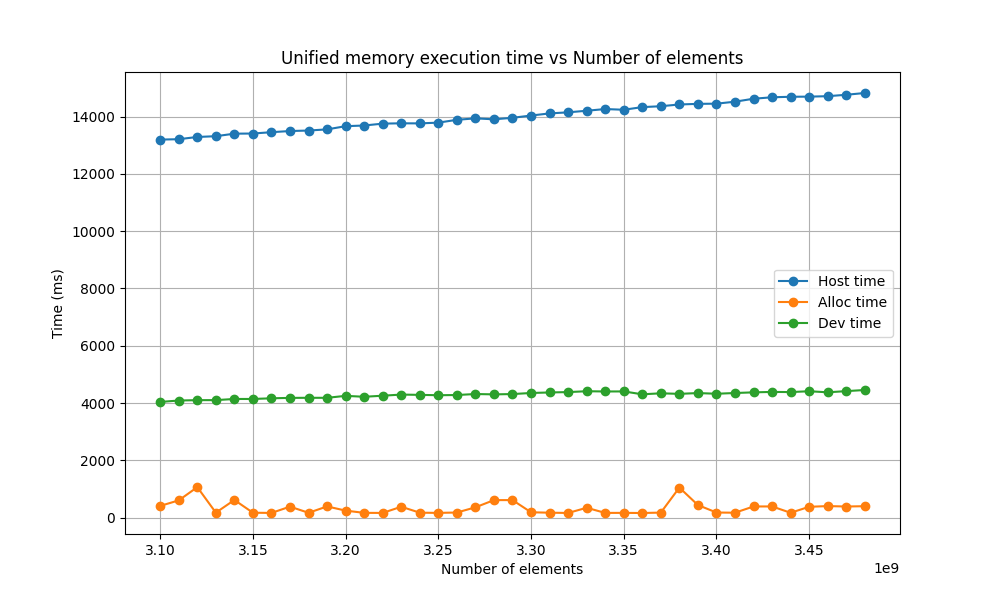
\includegraphics[width=0.9\textwidth]{./imagenes/P2_5/time_vs_elements.png}
				}
				\caption{Tiempo de ejecución en el \textit{host} y el \textit{device}.}
				\label{fig:time_vs_elements_5}
			\end{figure}

			\begin{figure}
				\centering
				\fbox{
					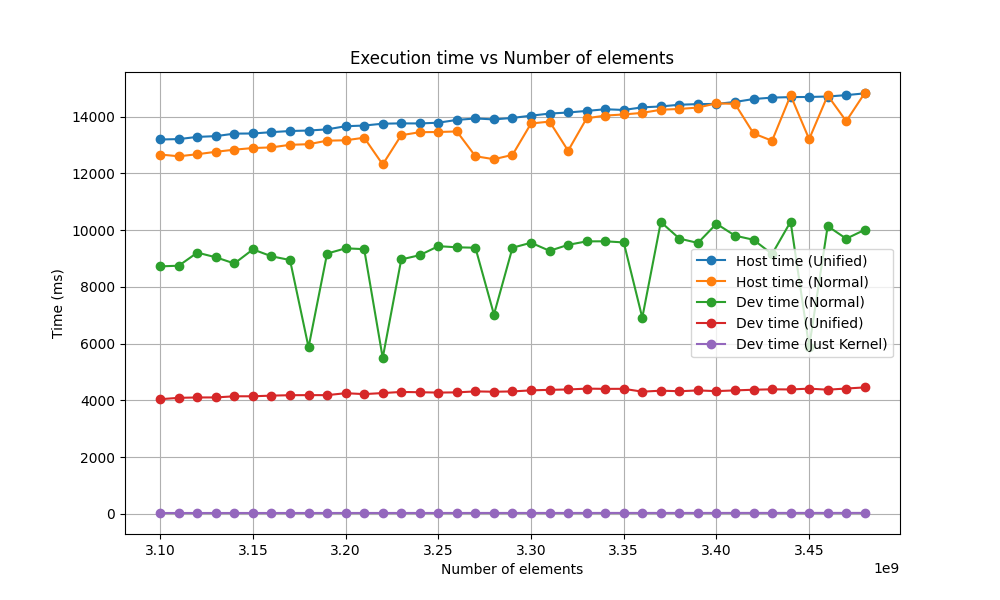
\includegraphics[width=0.9\textwidth]{./imagenes/P2_5/time_vs_elements_host.png}
				}
				\caption{\textit{Speedup} en función del número de elementos.}
				\label{fig:time_vs_elements_host_5}
			\end{figure}

		\subsubsection{Análisis de resultados}

			En este apartado se implementarán mejoras destinadas a optimizar el rendimiento observado en los experimentos previos. Para ello, se modificará el código original para utilizar memoria unificada. Como se analizó anteriormente, la transferencia de datos entre el \textit{host} y el dispositivo, ya sea de ida o de vuelta, representa una de las etapas más costosas en términos de tiempo, especialmente a medida que aumenta el número de elementos a transferir. Este factor impacta negativamente en los resultados y reduce la escalabilidad del problema. El uso de memoria unificada es una solución viable, ya que permite trabajar con un espacio de memoria único accesible tanto desde el \textit{host} como desde el dispositivo. Esto elimina la necesidad de transferir datos explícitamente entre ambos, lo que puede traducirse en una mejora significativa del rendimiento.

			Aunque la implementación de esta solución simplifica el desarrollo del programa al evitar la gestión manual de las transferencias de datos, es importante considerar el posible impacto en el rendimiento. La memoria unificada es una abstracción para el programador, pero internamente sigue dependiendo de la transferencia de datos, lo que puede introducir latencias en las operaciones de lectura y escritura. Por ello, resulta esencial evaluar el rendimiento de la solución con memoria unificada y compararlo con la versión original, para determinar si las ventajas en la transferencia de datos compensan las posibles pérdidas asociadas al uso de esta memoria.

			En la Figura \ref{fig:time_vs_elements_5} se presenta el tiempo de ejecución en el \textit{host} y en el dispositivo utilizando memoria unificada. Se observa un comportamiento similar al de los casos anteriores, donde el tiempo de ejecución en el dispositivo es significativamente menor que en el \textit{host}. Además, los tiempos de ejecución aumentan de forma lineal con el número de elementos, pero este incremento es mucho más pronunciado en el \textit{host}. Los resultados muestran que, mientras el \textit{host} mantiene un comportamiento similar al de los apartados previos, los tiempos en el dispositivo son notablemente menores, lo que sugiere que el uso de memoria unificada ha mejorado el rendimiento en el dispositivo.

			En la Figura \ref{fig:time_vs_elements_host_5} se comparan los tiempos obtenidos en las distintas partes del código para la solución con memoria unificada y para las versiones anteriores. Se aprecia que los tiempos en el \textit{host} con memoria unificada son ligeramente mayores que en las versiones previas, lo que indica que no se lograron mejoras significativas en el rendimiento del \textit{host}. Sin embargo, dado que las diferencias son mínimas, este deterioro puede considerarse despreciable y podría deberse a la latencia asociada con la gestión interna de la memoria unificada o a \textit{overheads} del sistema en el momento de las pruebas. Por otro lado, los resultados demuestran que la memoria unificada mejora los tiempos de ejecución en el dispositivo. Los tiempos en esta configuración son aproximadamente la mitad de los obtenidos cuando la transferencia de datos es gestionada manualmente por el programador. Además, el incremento en los tiempos a medida que aumenta el número de elementos es menor en comparación con las soluciones anteriores, lo que sugiere una mejora en la escalabilidad del problema.

			En base a los resultados obtenidos se pueden derivar las siguientes conclusiones:

			\begin{itemize}

				\item Las transferencias de datos entre el \textit{host} y el dispositivo son una de las fases que más tiempo consumen, especialmente la transferencia de datos de vuelta al \textit{host}.

				\item Las transferencias de datos siguen siendo necesarias en el caso de memoria unificada, aunque son gestionadas internamente por el sistema.

				\item El uso de memoria unificada ha permitido mejorar el rendimiento en el dispositivo, reduciendo los tiempos de ejecución en comparación con la solución original.

				\item El uso de memoria unificada ha permitido mejorar la escalabilidad del problema, reduciendo el incremento de los tiempos de ejecución conforme se aumenta el número de elementos.

				\item El uso de memoria unificada no ha permitido mejorar el rendimiento en el \textit{host}, aunque la diferencia en los tiempos obtenidos es despreciable.

				\item Los resultados obtenidos son consistentes con las expectativas previas y confirman la ventaja de la memoria unificada para tareas computacionales intensivas, aunque el tiempo de transferencia de datos sigue siendo un área por optimizar y a tener en cuenta.

			\end{itemize}

\section{Ejercicio 3}

	% TODO
	% Davido

\section{Conclusiones}

	% TODO
	% Davido

\begin{thebibliography}{9}
	\bibitem{cesga} CESGA, Centro de supercomputación de Galicia, \href{https://www.cesga.es/}{Enlace}.
\end{thebibliography}

\end{document}